\title{Systems Approach - Midterm}
\author{Ryan Spangler}
\date{\today}

\documentclass[10pt]{article}

\usepackage{commath}
\usepackage{graphicx}
\usepackage{listings}
\usepackage{amsfonts}

% python highlighting ----------
\usepackage{color}
\usepackage{listings}
\usepackage{textcomp}
\usepackage{setspace}
%\usepackage{palatino}

%\doublespacing

\setcounter{secnumdepth}{0}

\begin{document}
\maketitle

\section{Introduction}

For my midterm I chose to examine the nature of open source software projects.  Open source interests me for a variety of reasons.  I draw from a number of open source projects in my day to day life to get things done, and I am just now of the ability to start giving back to the community.  The collaborative nature of an OS project inspires me as an example of something founded on distributed, voluntarily contributing individuals.  Despite everyone's conflicting viewpoints and personal histories something unified and coherent (mostly) emerges.  It seems to me a perfect subject for systems inquiry.

\section{Methods}

I approached this subject with an eye towards what makes certain OS projects successful and others fail forgotten and alone.  Using systems methodology, I wanted to extract the defining feedback loops of the OS project system and examine them.  I drew inspiration from Checkland's seven step process, but really only applied the first couple (namely, 1-3 and 5).  I did not construct an ideal system first, as I did not know what the ideal system was.  In a way, OS works because it is the implementation of a certain ideal system.  I constructed a system with the relevant actors related in the ways I saw most influential towards one another, as a way to clarify my own thinking about what I thought an OS project was.  

I did run a preliminary CATWOE for the success of OS projects with the following results:

\begin{itemize}
\item C(ustomer) - Users of the software, companies or individuals.
\item A(ctors) - Contributors, people who develop and improve the project.
\item T(ransformation) - Turning needs into software solutions.
\item W(eltanschauung) - OS is a distributed means to coordinate contributions by many individuals.  Software should be free to use and modify.
\item O(wner) - In a real sense, everyone.
\item E(nvironment) - Other related libraries and projects, the larger economic reality.
\end{itemize}

\section{Process}

During step 2 I wrote out everything I could about the system.  I have several pages of notes with everything from descriptions to potential causes of failure to a list of successful and unsuccessful OS projects.  Getting everything out helped me to clarify what elements are most critical and how they relate to everything else.  

From the raw materials of step 2 I extracted the key components of the system.  The process of defining the elements (Checkland step 3) was most illuminating.  I found I had to ignore a great amount of detail in order to hone in on the essential contributors to the system.  The elements that survived this process were 

\begin{itemize}
\item Projects - the actual software and codebase.
\item Contributors - the people contributing to the project.
\item Users - whoever uses the project.
\item Related Projects - other projects that either support or depend on this project.
\item Need - the original need that compels the contributors to start and continue development on the project.
\item Available Time - how much time contributors or users have to spend with the software.
\item Other Priorities - other things that must be accomplished unrelated to the project.
\end{itemize}

These I arranged into a diagram outlining the relationships each has to each other, whether they reinforce or inhibit one another and what the nature of the relationship was.  This diagram I then examined to identify feedback loops in order to discern what kinds of system effects might lead to the persistence or sustaining of the project activity, and conversely what could lead to their downfall.

\section{Diagram}

\begin{center}
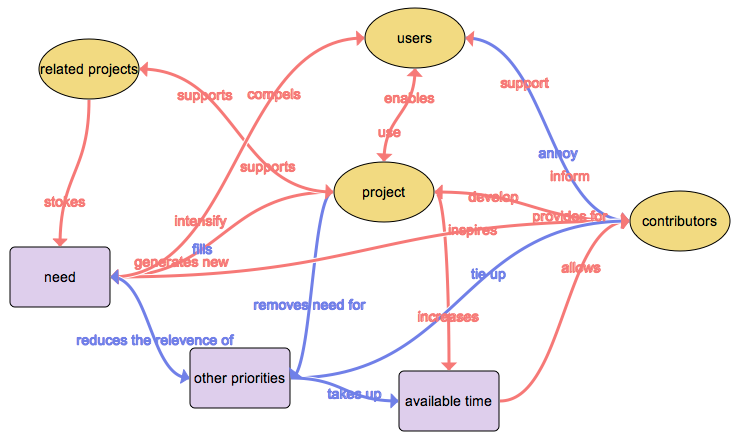
\includegraphics[scale=0.6]{clear.png}
\end{center}

In this diagram the yellow circles are concrete actors, whereas the lavender rectangles are more conceptual influences.  Red arrows are positive influences while blue arrows are negative ones.  There is a description for each component as well as a description of each relationship.  For clarity, each arrow label is closer to its target, so for bidirectional relationships you can discern which influence goes which direction.  I tried my best to untangle the diagram but there is still some ambiguity remaining.  For the most part though the relationships can be discerned.

\section{Discussion}

From the diagram a number of important feedback loops can be identified and reflected on.  Everything flows originally from need, which inspires the contributors to start developing the project.  The project relies on all three of the other components to grow beyond this initial stage.  It requires support from other projects which it depends on and requires continual input from one or some contributors.  Once the project gets going it provides for contributors and users, while in return supporting those projects which support it (by increasing their relevance and application).  All of these feed into one another.

One potential source of failure in an OS is that the existence of the project fills the original need, and so no one worries about extending it.  In this case the project could survive, but it would not thrive and would eventually be replaced.

The lavender subsystem shows how other priorities can impact available time.  The project could be abandoned entirely if other priorities are strong enough, even if other factors are present.  However, the project itself can remove the need for other priorities, by replacing them with automated solutions for instance.  In this case the project is again supporting its own existence by removing potentially inhibitory influences.  Also, the stronger the need, the less other priorities matter, thereby increasing the investment into the project through contributor time.  

The most critical loop I identified from the diagram was the direct reinforcing cycle between projects and other related projects.  This network effect builds on itself by providing the means for the improvement of one project to by surrogate improve all related projects.  This amplifying feedback loop is one of the most powerful, with simple projects getting swept into mainstream by association with a strong emerging project.

\section{Conclusion}

The process I went through was insightful to the inner workings of the system.  I feel the model could be pared down even further, for instance by combining available time with other priorities.  I find the identification of causal feedback loops (and whether inhibitory or excitatory) to be indispensible in the quest for true system clarity.  Even in a system with as few elements as this the combinations of paths and the tracing of effects exposed a great deal of richness in its dynamics.  I feel I could spend much more time simply following the implications of the structure demonstrated in the diagram.  The next step would be to apply this model to various real projects and eliminate flaws in the structure of the system as given when compared to real world scenarios, or generalize this model to incorporate more real world variety.  

\end{document}  

